\chapter{Arquitetura distribuída}
\label{chap:arquitetura-distribuida}



\section{Projeto conceitual}
\begin{figure}[ht]
    \centering
    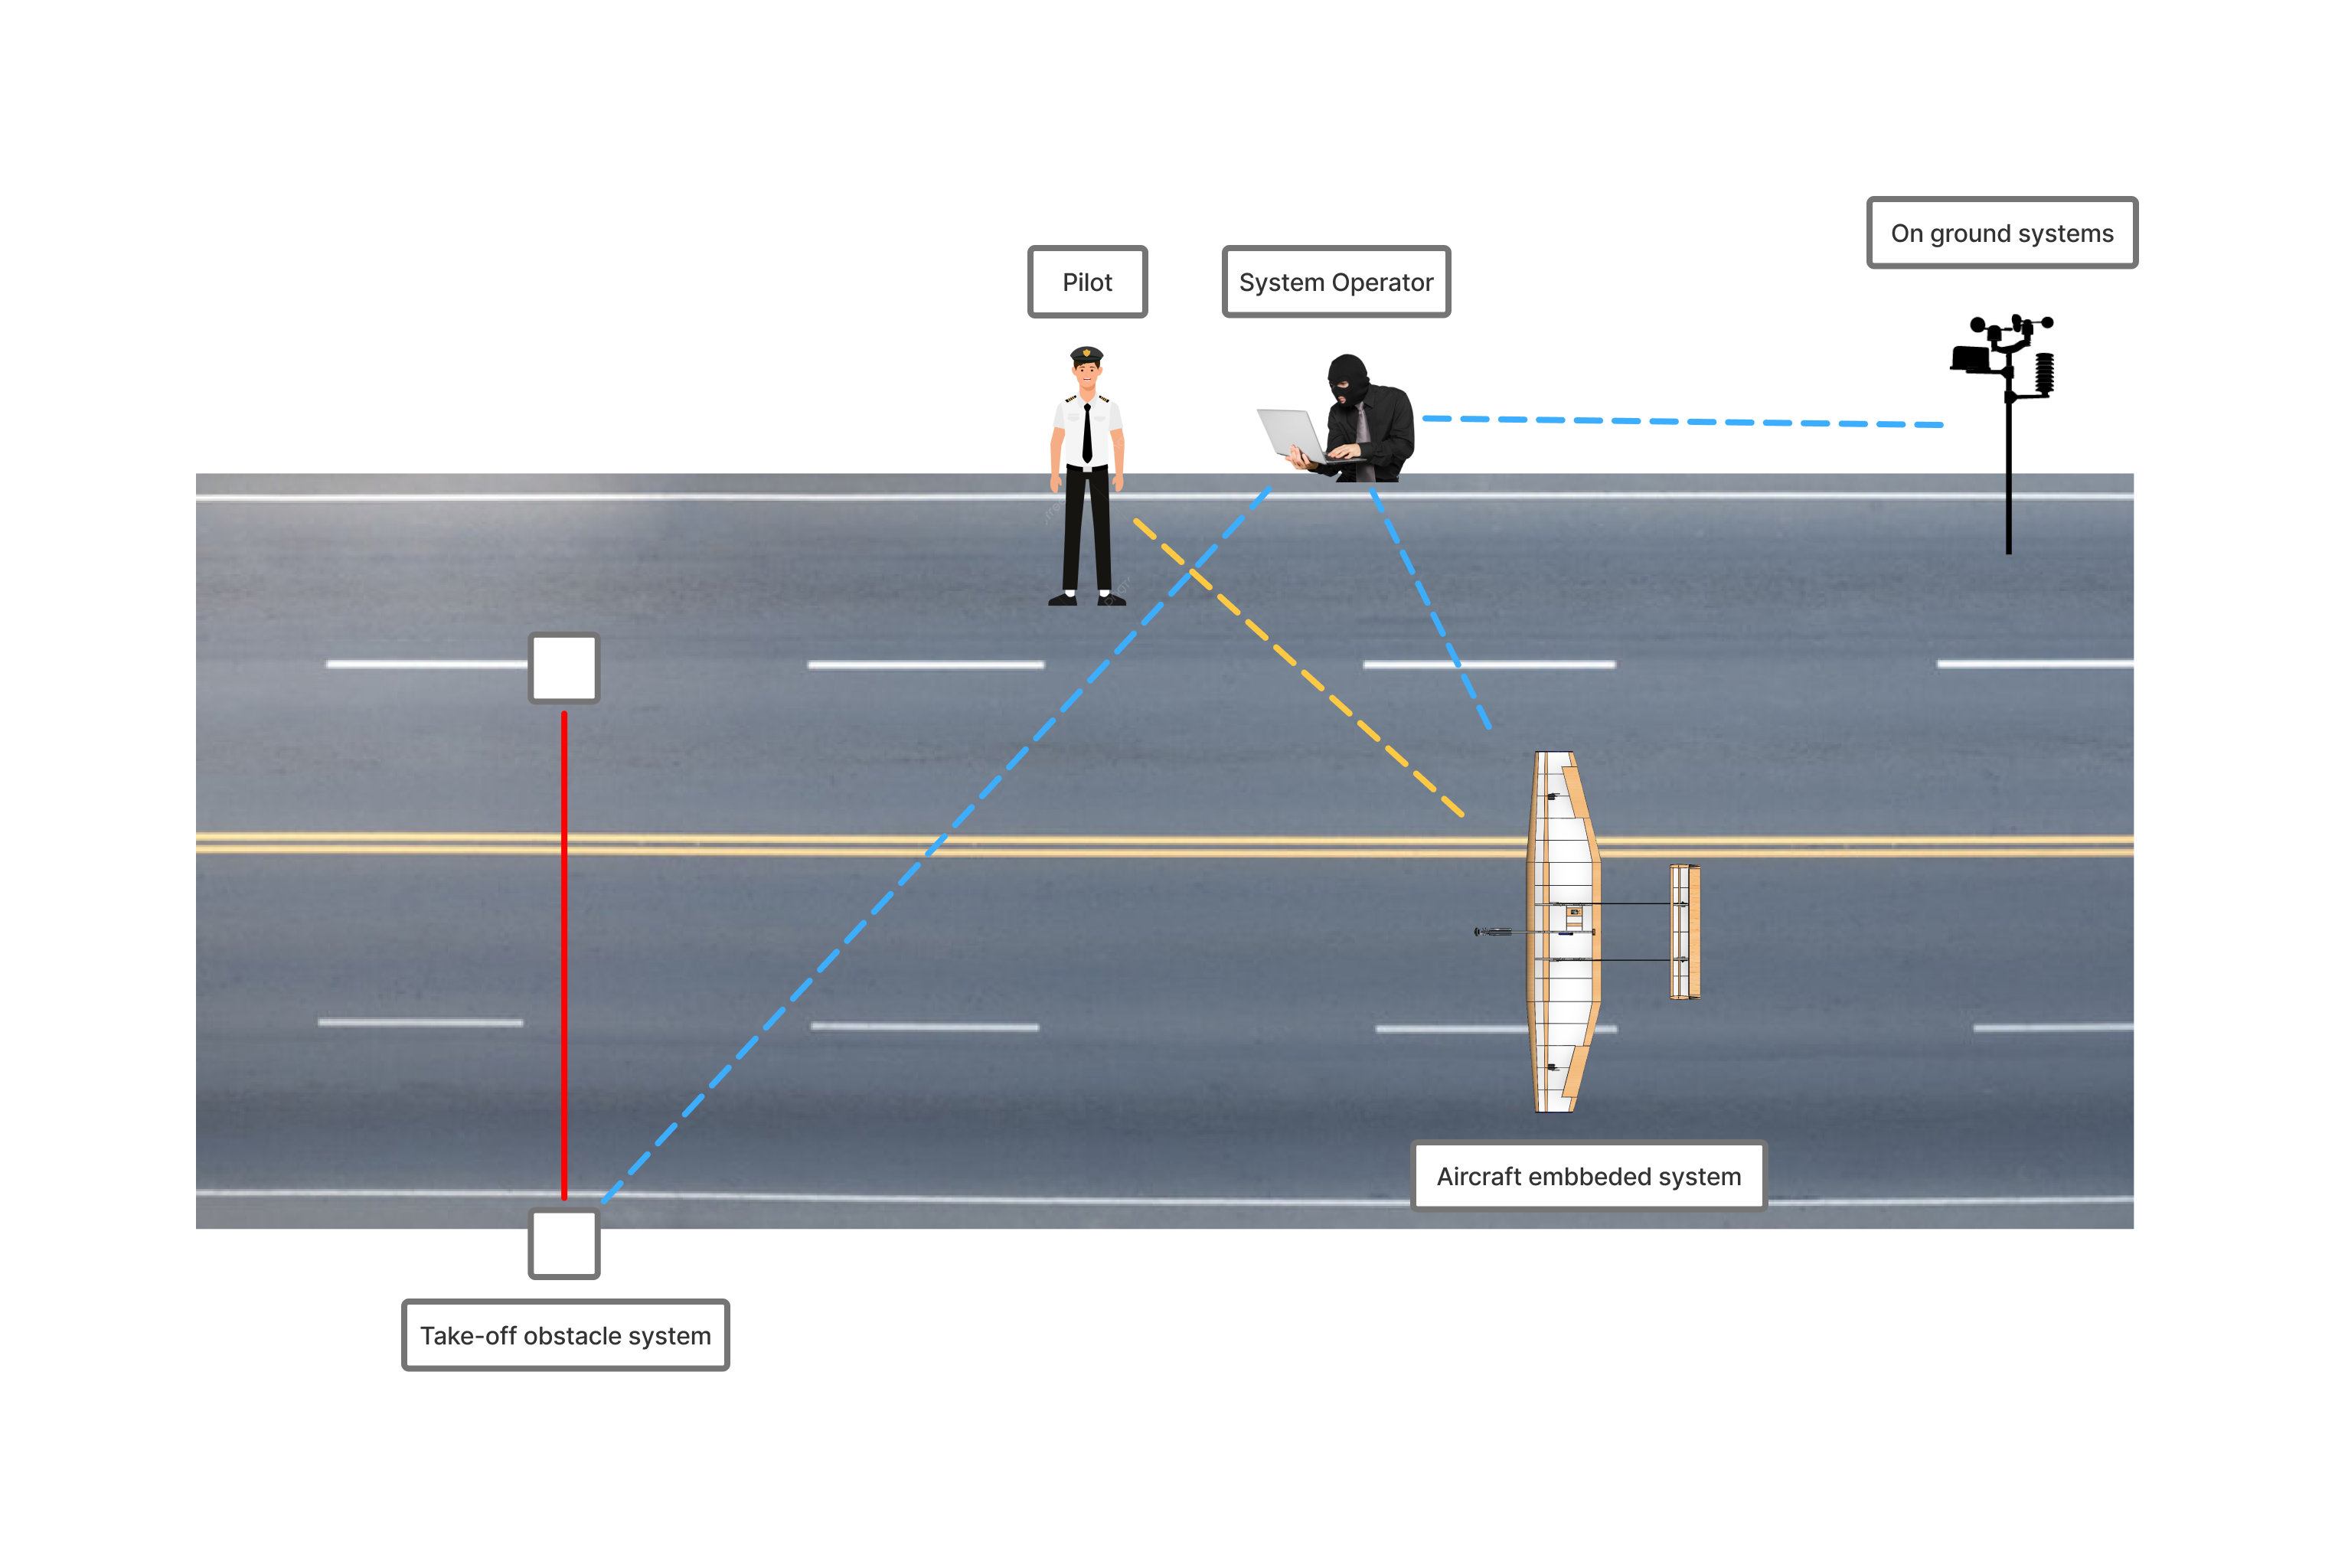
\includegraphics[width=0.9\textwidth]{images/design_conceitual.png}
    \caption{\textit{Design} conceitual da solução}
    \label{fig:design-conceitual}
\end{figure}

\section{Arquitetura de comunicação}
(Diagrama que se completa ao longo das subsections)

\subsection{Componentes distribuídos}
Ponta, middleware e client

\begin{figure}[ht]
    \centering
    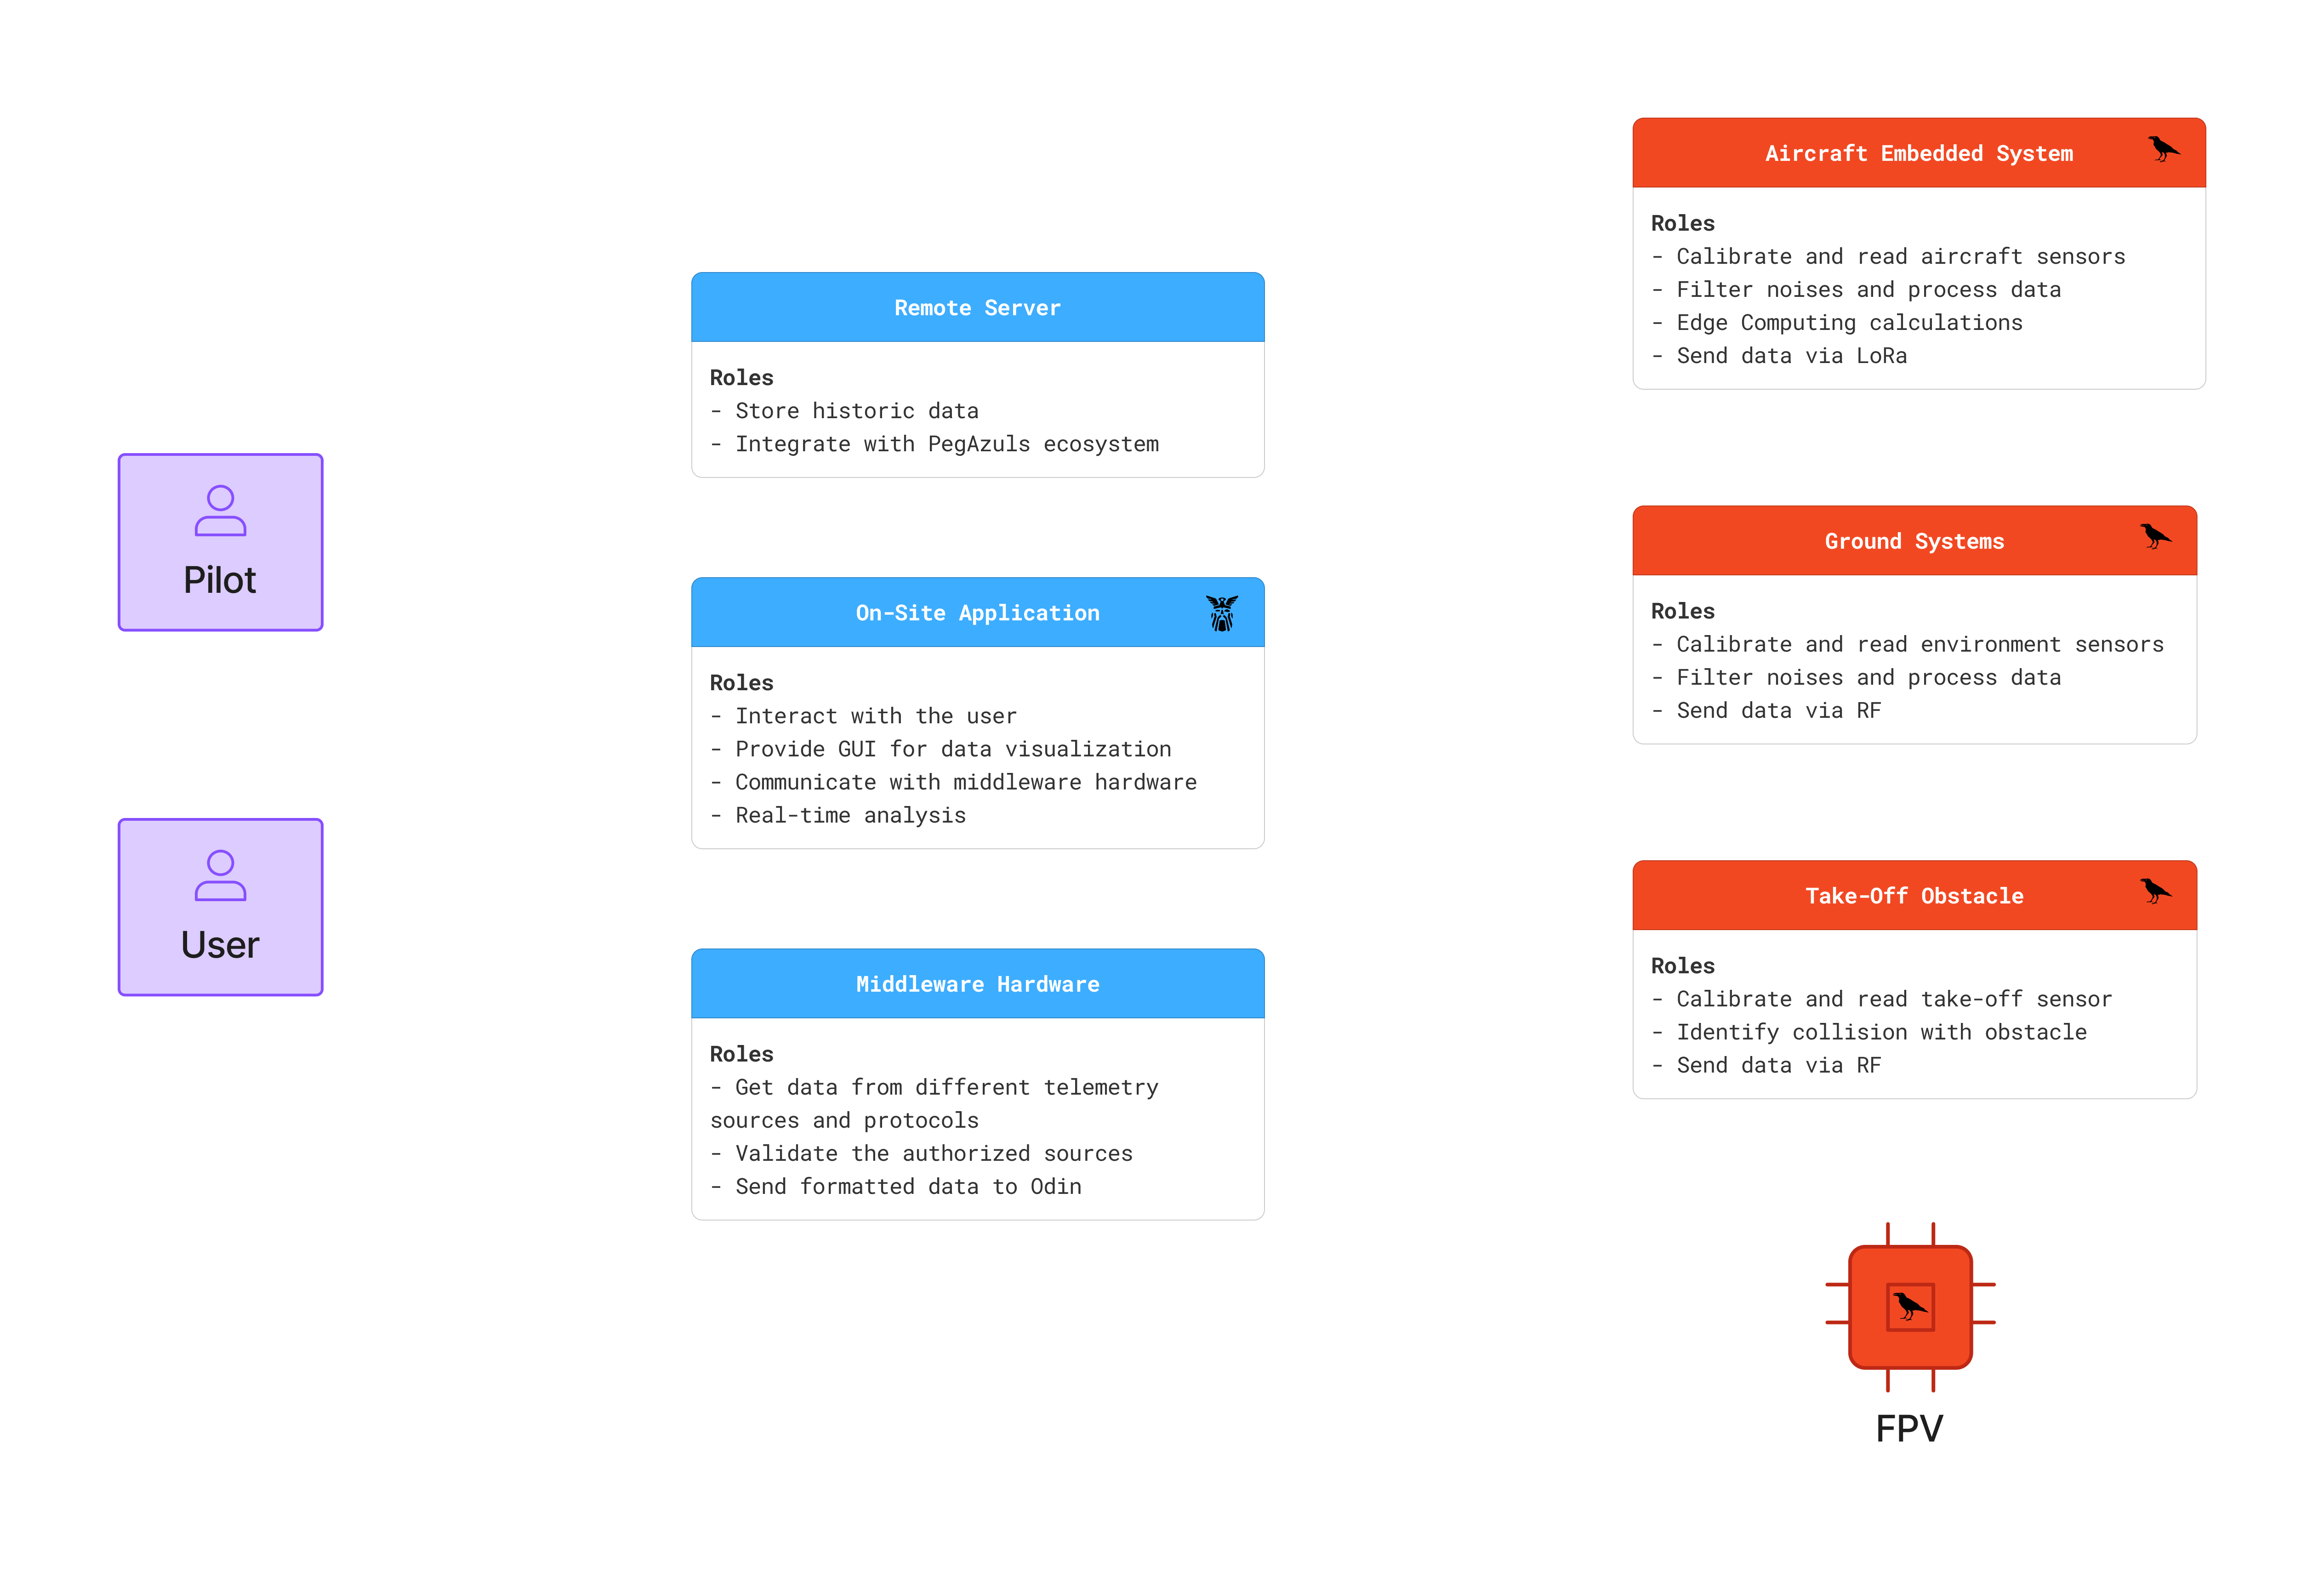
\includegraphics[width=0.85\textwidth]{images/componentes_design_comunicacao.png}
    \caption{Componentes distribuidos}
    \label{fig:componentes-distribuidos}
\end{figure}

\subsection{Camada física}
Escolha da antena e módulo RF

\begin{figure}[ht]
    \centering
    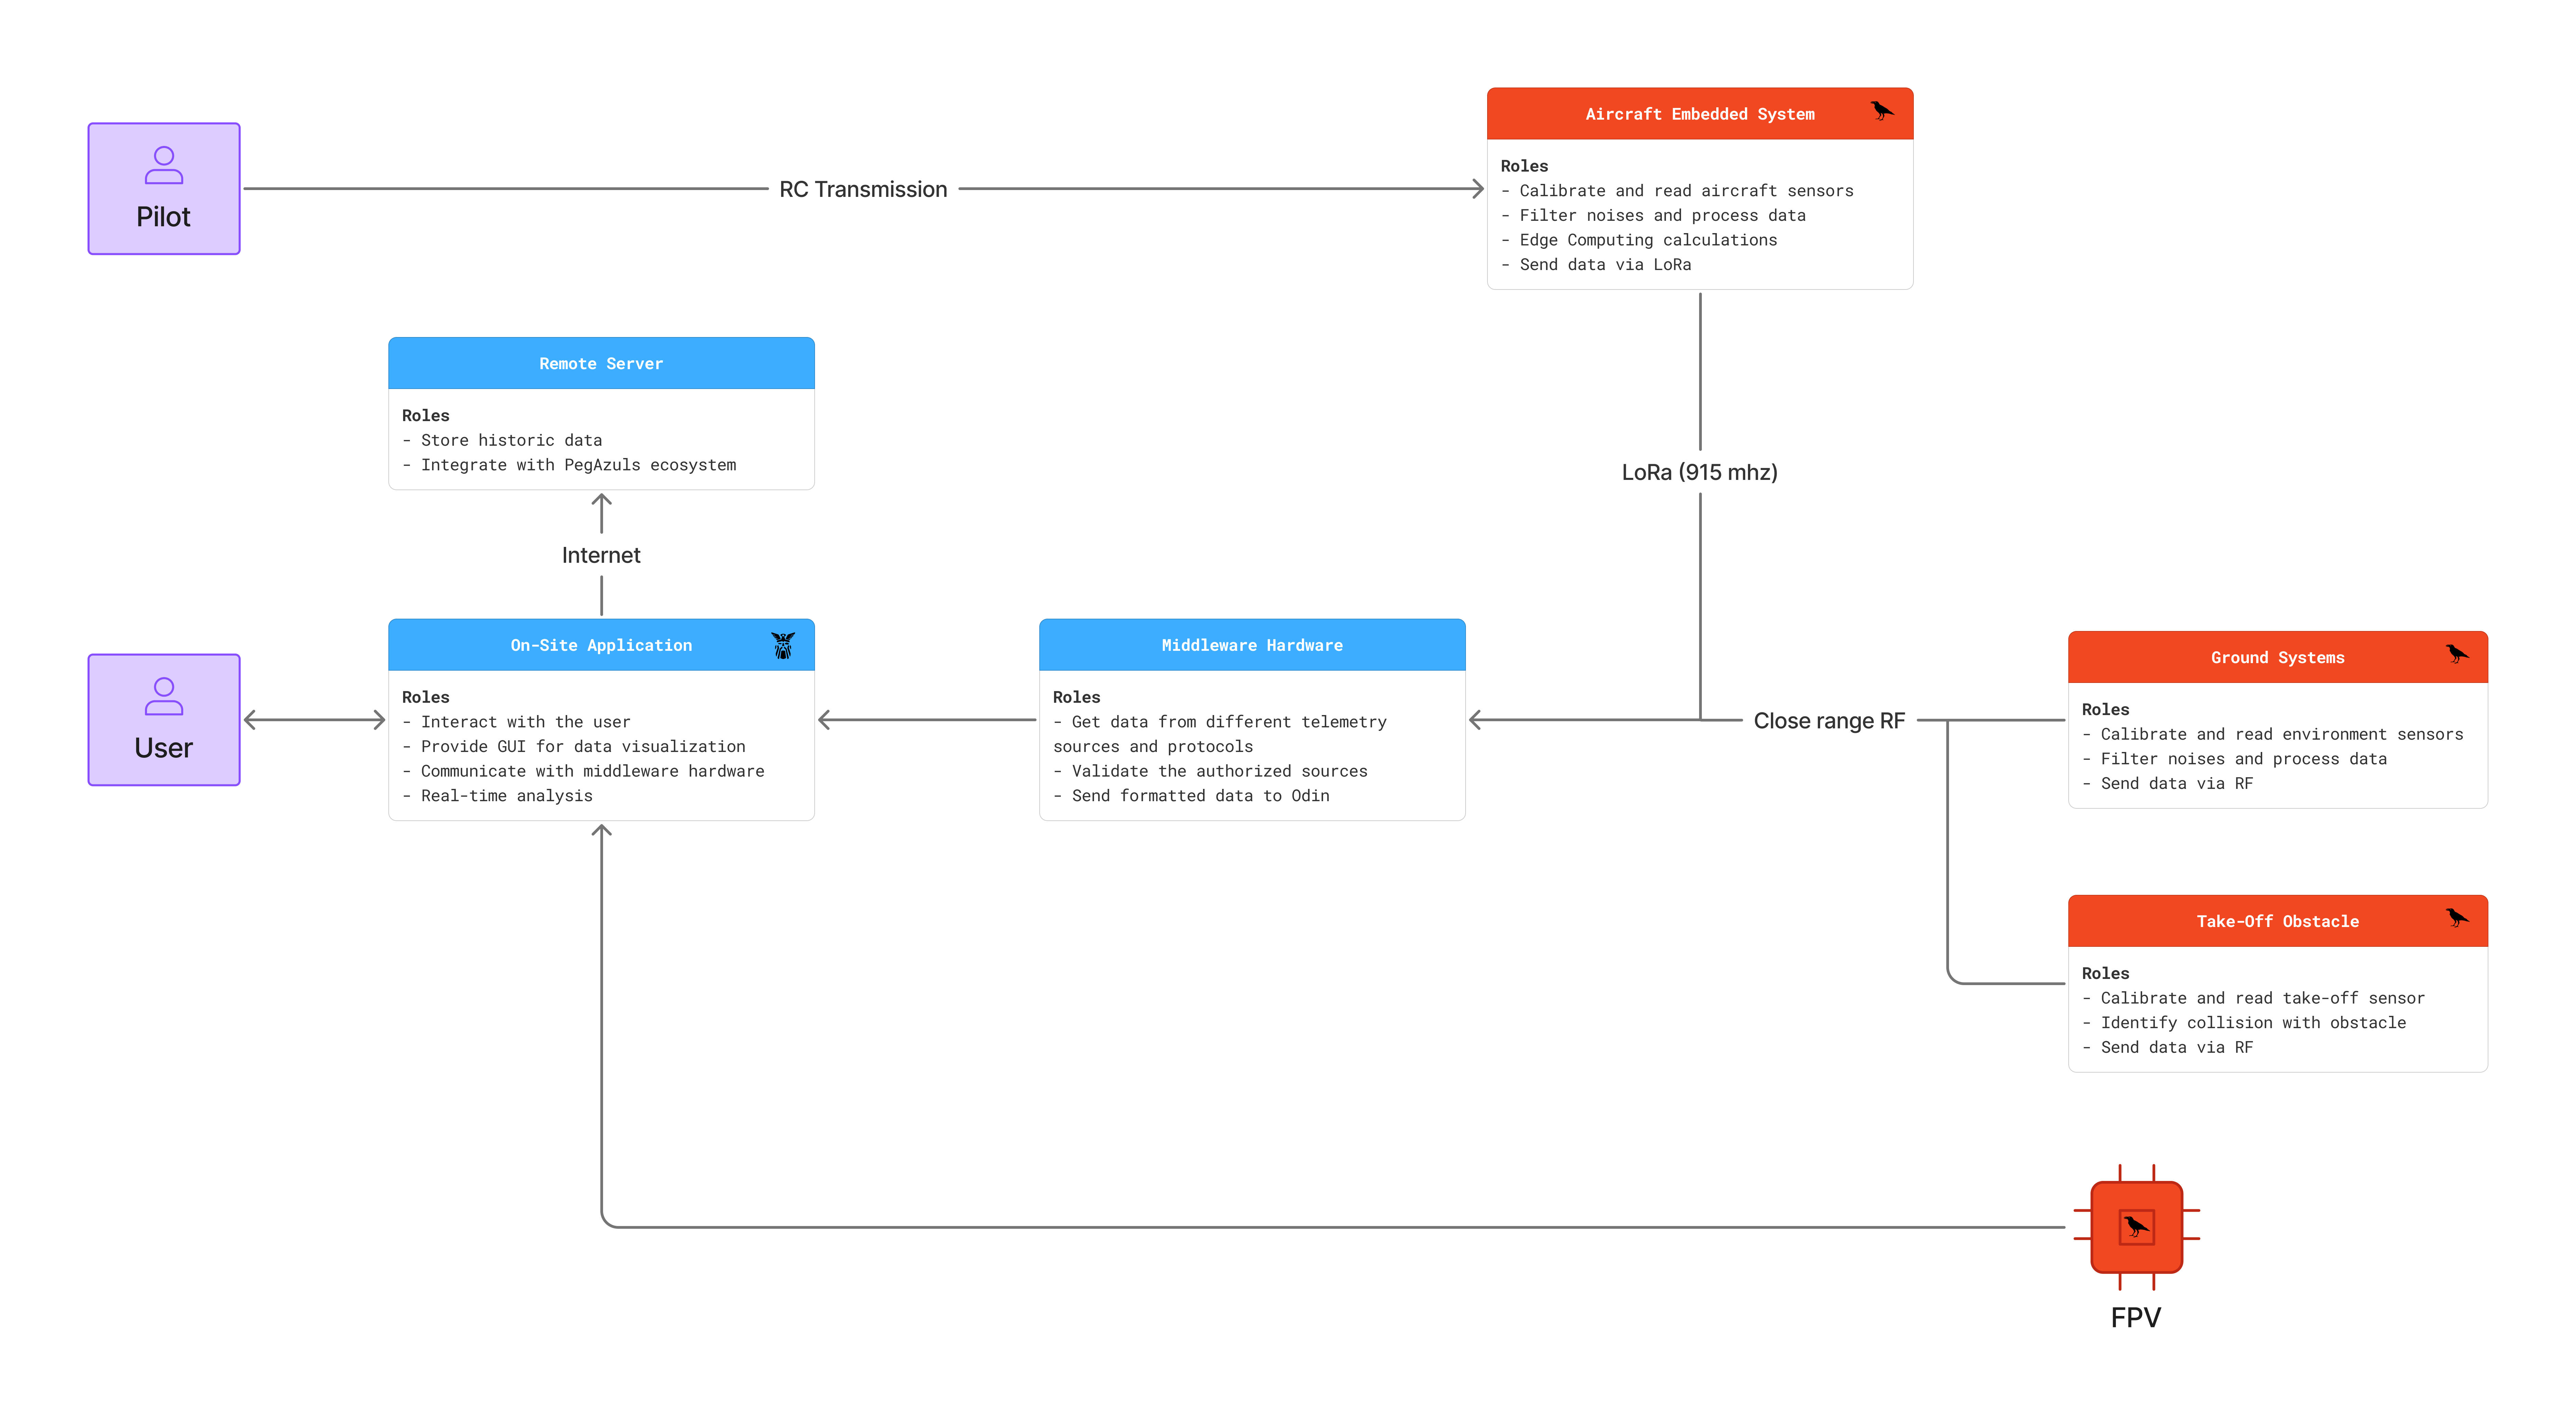
\includegraphics[width=0.85\textwidth]{images/camada_fisica_design_comunicacao.png}
    \caption{Camada física do sistema}
    \label{fig:camada-fisica}
\end{figure}

\subsection{Camada de transporte}
Escolha dos protocolos

\begin{figure}[ht]
    \centering
    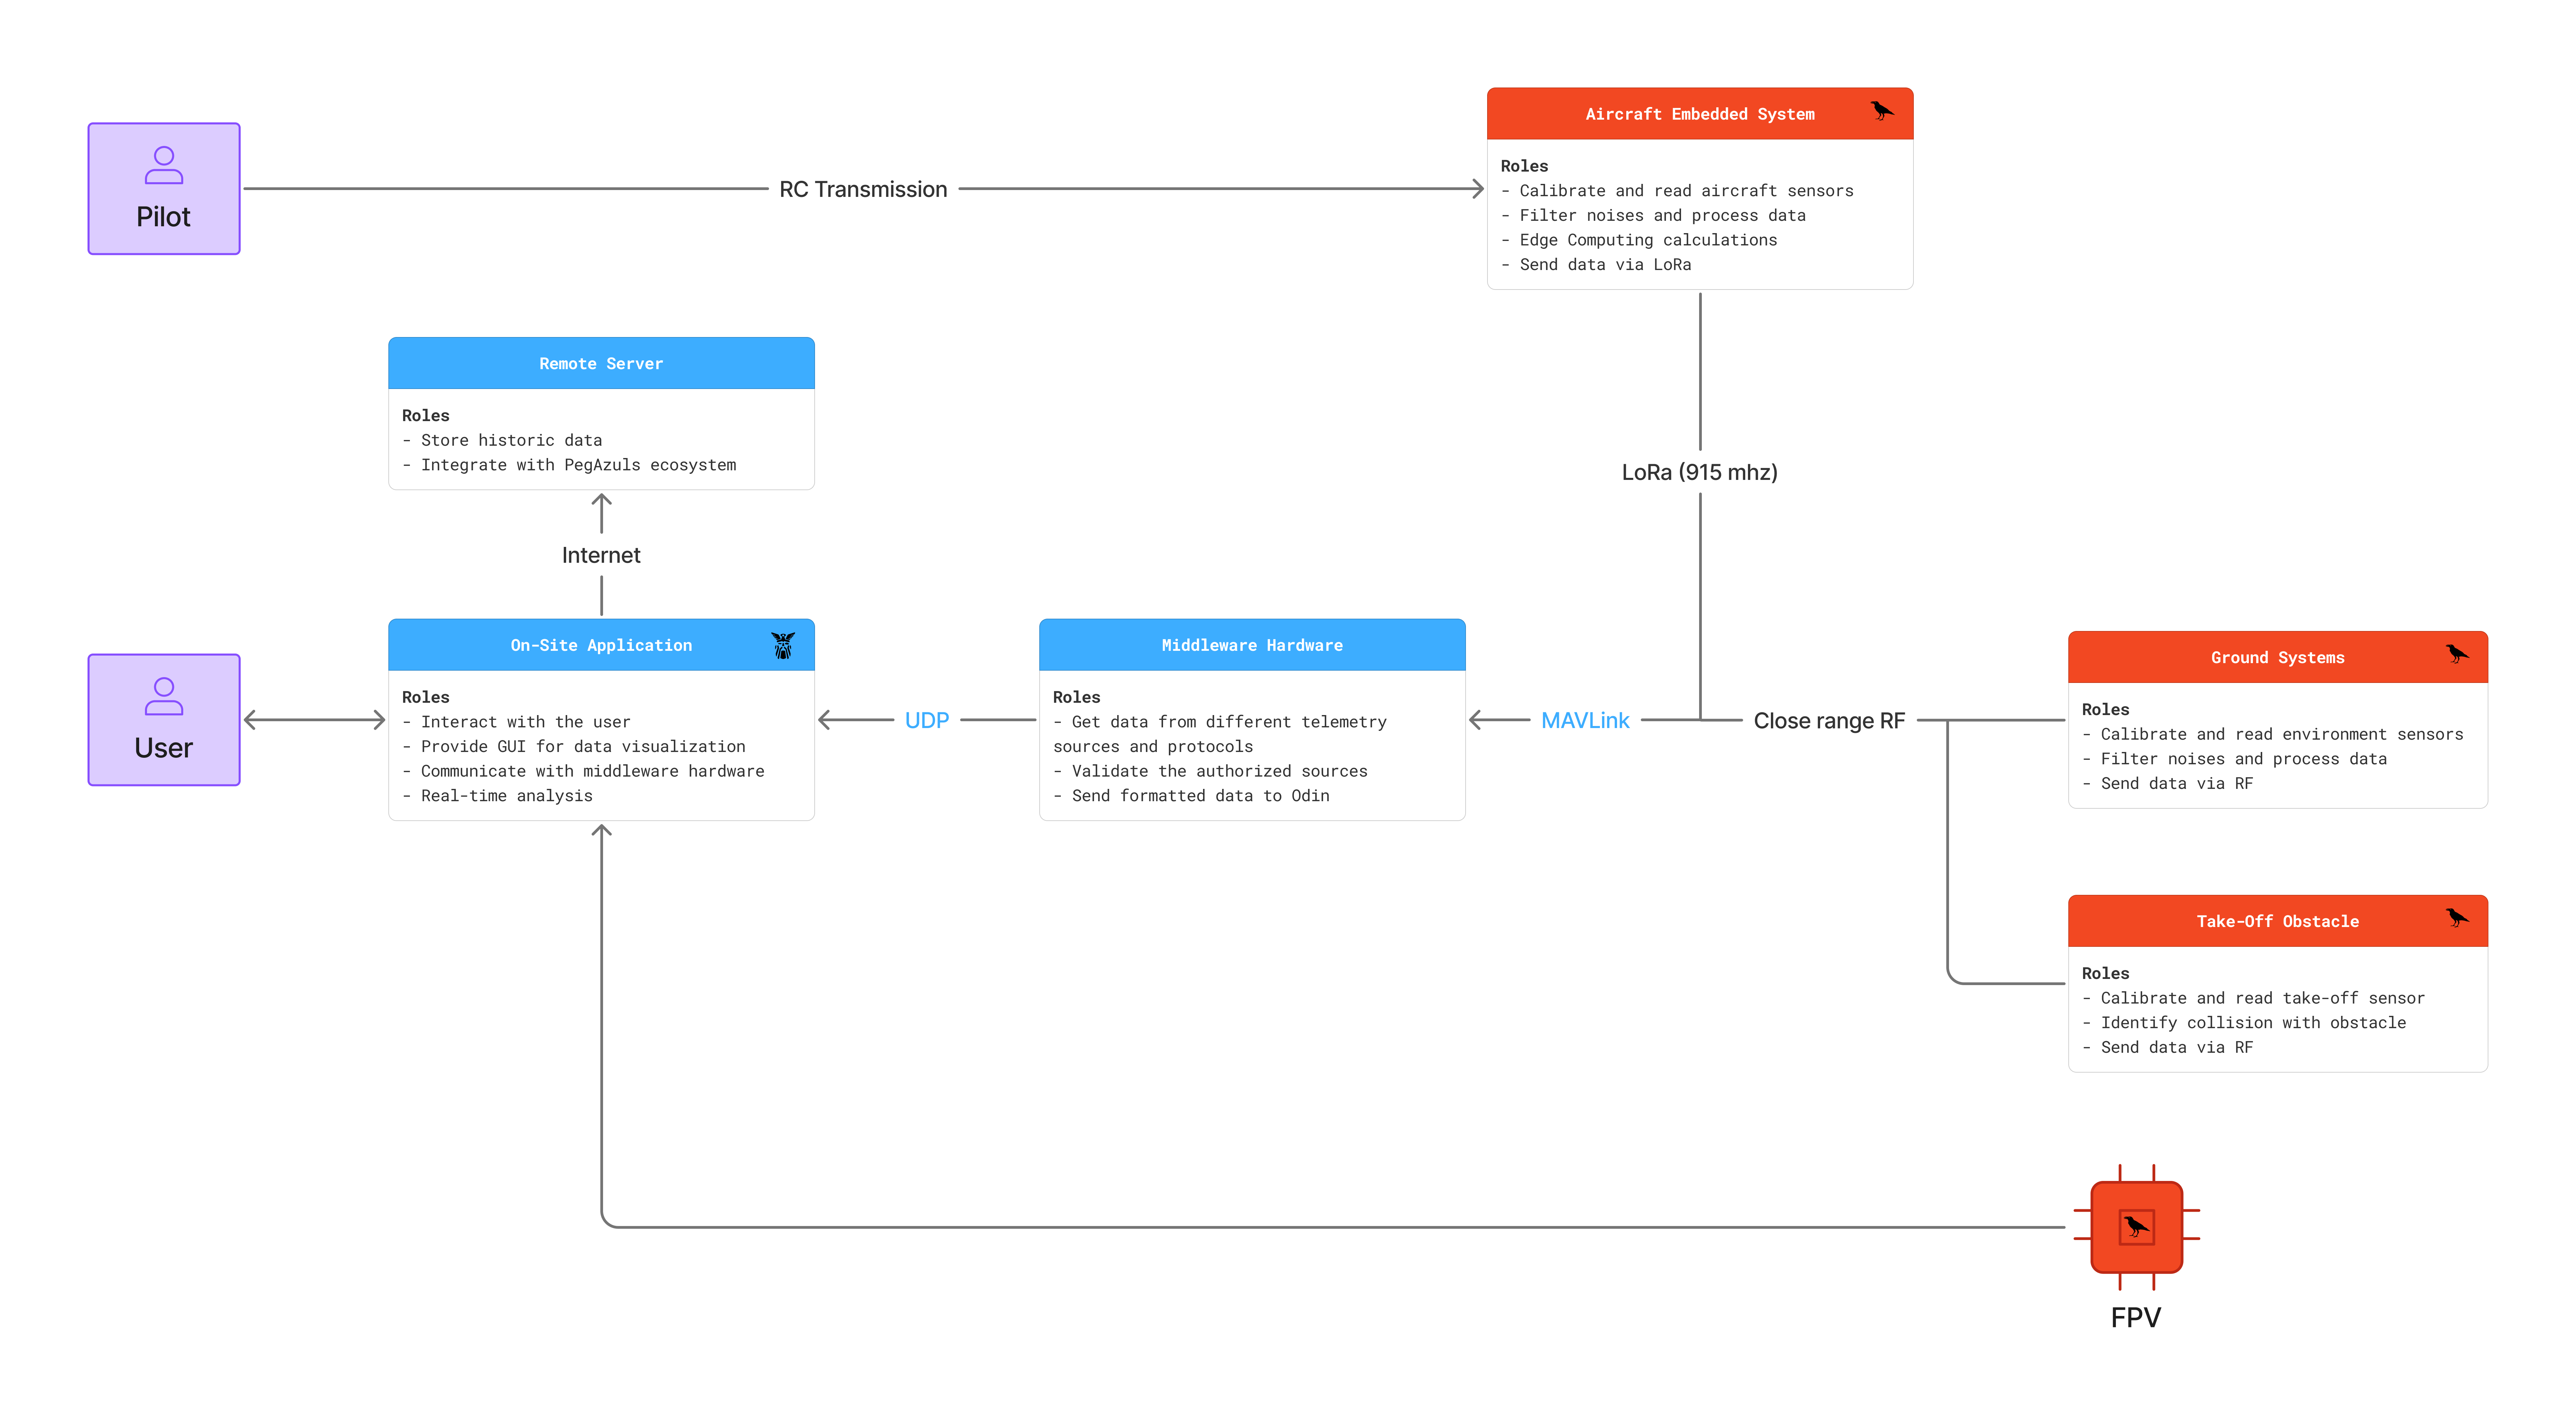
\includegraphics[width=0.85\textwidth]{images/design_de_comunicacao.png}
    \caption{\textit{Design} de comunicação}
    \label{fig:design-de-comunicacao}
\end{figure}

